\documentclass[]{article}
\usepackage{lmodern}
\usepackage{amssymb,amsmath}
\usepackage{ifxetex,ifluatex}
\usepackage{fixltx2e} % provides \textsubscript
\ifnum 0\ifxetex 1\fi\ifluatex 1\fi=0 % if pdftex
  \usepackage[T1]{fontenc}
  \usepackage[utf8]{inputenc}
\else % if luatex or xelatex
  \ifxetex
    \usepackage{mathspec}
  \else
    \usepackage{fontspec}
  \fi
  \defaultfontfeatures{Ligatures=TeX,Scale=MatchLowercase}
\fi
% use upquote if available, for straight quotes in verbatim environments
\IfFileExists{upquote.sty}{\usepackage{upquote}}{}
% use microtype if available
\IfFileExists{microtype.sty}{%
\usepackage[]{microtype}
\UseMicrotypeSet[protrusion]{basicmath} % disable protrusion for tt fonts
}{}
\PassOptionsToPackage{hyphens}{url} % url is loaded by hyperref
\usepackage[unicode=true]{hyperref}
\hypersetup{
            pdftitle={Perinatal malnutrition in male mice influences gene expression in the next generation offspring: Potential role of epigenetics.},
            pdfauthor={Ana Isabel del Val},
            pdfborder={0 0 0},
            breaklinks=true}
\urlstyle{same}  % don't use monospace font for urls
\usepackage[margin=2cm]{geometry}
\usepackage{color}
\usepackage{fancyvrb}
\newcommand{\VerbBar}{|}
\newcommand{\VERB}{\Verb[commandchars=\\\{\}]}
\DefineVerbatimEnvironment{Highlighting}{Verbatim}{commandchars=\\\{\}}
% Add ',fontsize=\small' for more characters per line
\usepackage{framed}
\definecolor{shadecolor}{RGB}{248,248,248}
\newenvironment{Shaded}{\begin{snugshade}}{\end{snugshade}}
\newcommand{\KeywordTok}[1]{\textcolor[rgb]{0.13,0.29,0.53}{\textbf{#1}}}
\newcommand{\DataTypeTok}[1]{\textcolor[rgb]{0.13,0.29,0.53}{#1}}
\newcommand{\DecValTok}[1]{\textcolor[rgb]{0.00,0.00,0.81}{#1}}
\newcommand{\BaseNTok}[1]{\textcolor[rgb]{0.00,0.00,0.81}{#1}}
\newcommand{\FloatTok}[1]{\textcolor[rgb]{0.00,0.00,0.81}{#1}}
\newcommand{\ConstantTok}[1]{\textcolor[rgb]{0.00,0.00,0.00}{#1}}
\newcommand{\CharTok}[1]{\textcolor[rgb]{0.31,0.60,0.02}{#1}}
\newcommand{\SpecialCharTok}[1]{\textcolor[rgb]{0.00,0.00,0.00}{#1}}
\newcommand{\StringTok}[1]{\textcolor[rgb]{0.31,0.60,0.02}{#1}}
\newcommand{\VerbatimStringTok}[1]{\textcolor[rgb]{0.31,0.60,0.02}{#1}}
\newcommand{\SpecialStringTok}[1]{\textcolor[rgb]{0.31,0.60,0.02}{#1}}
\newcommand{\ImportTok}[1]{#1}
\newcommand{\CommentTok}[1]{\textcolor[rgb]{0.56,0.35,0.01}{\textit{#1}}}
\newcommand{\DocumentationTok}[1]{\textcolor[rgb]{0.56,0.35,0.01}{\textbf{\textit{#1}}}}
\newcommand{\AnnotationTok}[1]{\textcolor[rgb]{0.56,0.35,0.01}{\textbf{\textit{#1}}}}
\newcommand{\CommentVarTok}[1]{\textcolor[rgb]{0.56,0.35,0.01}{\textbf{\textit{#1}}}}
\newcommand{\OtherTok}[1]{\textcolor[rgb]{0.56,0.35,0.01}{#1}}
\newcommand{\FunctionTok}[1]{\textcolor[rgb]{0.00,0.00,0.00}{#1}}
\newcommand{\VariableTok}[1]{\textcolor[rgb]{0.00,0.00,0.00}{#1}}
\newcommand{\ControlFlowTok}[1]{\textcolor[rgb]{0.13,0.29,0.53}{\textbf{#1}}}
\newcommand{\OperatorTok}[1]{\textcolor[rgb]{0.81,0.36,0.00}{\textbf{#1}}}
\newcommand{\BuiltInTok}[1]{#1}
\newcommand{\ExtensionTok}[1]{#1}
\newcommand{\PreprocessorTok}[1]{\textcolor[rgb]{0.56,0.35,0.01}{\textit{#1}}}
\newcommand{\AttributeTok}[1]{\textcolor[rgb]{0.77,0.63,0.00}{#1}}
\newcommand{\RegionMarkerTok}[1]{#1}
\newcommand{\InformationTok}[1]{\textcolor[rgb]{0.56,0.35,0.01}{\textbf{\textit{#1}}}}
\newcommand{\WarningTok}[1]{\textcolor[rgb]{0.56,0.35,0.01}{\textbf{\textit{#1}}}}
\newcommand{\AlertTok}[1]{\textcolor[rgb]{0.94,0.16,0.16}{#1}}
\newcommand{\ErrorTok}[1]{\textcolor[rgb]{0.64,0.00,0.00}{\textbf{#1}}}
\newcommand{\NormalTok}[1]{#1}
\usepackage{graphicx,grffile}
\makeatletter
\def\maxwidth{\ifdim\Gin@nat@width>\linewidth\linewidth\else\Gin@nat@width\fi}
\def\maxheight{\ifdim\Gin@nat@height>\textheight\textheight\else\Gin@nat@height\fi}
\makeatother
% Scale images if necessary, so that they will not overflow the page
% margins by default, and it is still possible to overwrite the defaults
% using explicit options in \includegraphics[width, height, ...]{}
\setkeys{Gin}{width=\maxwidth,height=\maxheight,keepaspectratio}
\IfFileExists{parskip.sty}{%
\usepackage{parskip}
}{% else
\setlength{\parindent}{0pt}
\setlength{\parskip}{6pt plus 2pt minus 1pt}
}
\setlength{\emergencystretch}{3em}  % prevent overfull lines
\providecommand{\tightlist}{%
  \setlength{\itemsep}{0pt}\setlength{\parskip}{0pt}}
\setcounter{secnumdepth}{0}
% Redefines (sub)paragraphs to behave more like sections
\ifx\paragraph\undefined\else
\let\oldparagraph\paragraph
\renewcommand{\paragraph}[1]{\oldparagraph{#1}\mbox{}}
\fi
\ifx\subparagraph\undefined\else
\let\oldsubparagraph\subparagraph
\renewcommand{\subparagraph}[1]{\oldsubparagraph{#1}\mbox{}}
\fi

% set default figure placement to htbp
\makeatletter
\def\fps@figure{htbp}
\makeatother

\usepackage{etoolbox}
\makeatletter
\providecommand{\subtitle}[1]{% add subtitle to \maketitle
  \apptocmd{\@title}{\par {\large #1 \par}}{}{}
}
\makeatother
\usepackage{booktabs}
\usepackage{longtable}
\usepackage{array}
\usepackage{multirow}
\usepackage{wrapfig}
\usepackage{float}
\usepackage{colortbl}
\usepackage{pdflscape}
\usepackage{tabu}
\usepackage{threeparttable}
\usepackage{threeparttablex}
\usepackage[normalem]{ulem}
\usepackage{makecell}
\usepackage{xcolor}

\title{Perinatal malnutrition in male mice influences gene expression in the
next generation offspring: Potential role of epigenetics.}
\providecommand{\subtitle}[1]{}
\subtitle{Análisis de datos ómicos}
\author{Ana Isabel del Val}
\date{11 de abril, 2020}

\begin{document}
\maketitle

{
\setcounter{tocdepth}{3}
\tableofcontents
}
``

\subsection{Abstract}\label{abstract}

The dataset for the exercise is available at the entry Series GSE55304
of the in Gene Expression Omnibus.

This code is already sync with
\textbf{\emph{\href{https://github.com/AnadelVal/epigeneticsGSE55304}{github
repository}}}, which is public.

\textbf{\emph{\href{https://www.ncbi.nlm.nih.gov/geo/query/acc.cgi?acc=GSE55304}{This
is the source reference}}}.

\subsection{Objectives}\label{objectives}

It consists on determining whether patterns of gene expression in the
first generation offspring are also present in the following generation
offspring, via the paternal lineage. Paternal transmission of patterns
of gene expression strongly suggest epigenetic inheritance of disease
risk.

\subsection{Materials and methods}\label{materials-and-methods}

\subsubsection{Data source and experiment
design}\label{data-source-and-experiment-design}

Liver tissue was obtained from the following experimental groups:

\begin{itemize}
\item
  \begin{enumerate}
  \def\labelenumi{\alph{enumi})}
  \tightlist
  \item
    control male mice
  \end{enumerate}
\item
  \begin{enumerate}
  \def\labelenumi{\alph{enumi})}
  \setcounter{enumi}{1}
  \tightlist
  \item
    adult male mice previously exposed to 50\% caloric restriction in
    utero (IUGR)
  \end{enumerate}
\item
  \begin{enumerate}
  \def\labelenumi{\alph{enumi})}
  \setcounter{enumi}{2}
  \tightlist
  \item
    adult male mice overfed during lactation (ON)
  \end{enumerate}
\item
  \begin{enumerate}
  \def\labelenumi{\alph{enumi})}
  \setcounter{enumi}{3}
  \tightlist
  \item
    adult male offspring from control mice
  \end{enumerate}
\item
  \begin{enumerate}
  \def\labelenumi{\alph{enumi})}
  \setcounter{enumi}{4}
  \tightlist
  \item
    adult male offspring from IUGR mice
  \end{enumerate}
\item
  \begin{enumerate}
  \def\labelenumi{\alph{enumi})}
  \setcounter{enumi}{5}
  \tightlist
  \item
    adult male offspring from ON mice.
  \end{enumerate}
\end{itemize}

RNA was extracted and processed for further hybridization on Affymetrix
microarrays (GeneChip Mouse Genome 430 2.0 (Affymetrix, Santa Clara,
CA)).

Targets have been created manually and is composed by 5 groups, 3 arrays
in each group.

\begin{Shaded}
\begin{Highlighting}[]
\NormalTok{targets}
\end{Highlighting}
\end{Shaded}

\begin{verbatim}
##      FileName       Group  Genotype Treatment    ShortName
## 1  GSM1333830 BothControl      Both   Control BothControl1
## 2  GSM1333831 BothControl      Both   Control BothControl2
## 3  GSM1333832 BothControl      Both   Control BothControl3
## 4  GSM1333833   AdultIUGR     Adult      IUGR   AdultIUGR1
## 5  GSM1333834   AdultIUGR     Adult      IUGR   AdultIUGR2
## 6  GSM1333835   AdultIUGR     Adult      IUGR   AdultIUGR3
## 7  GSM1333836   AdultLact     Adult lactation   AdultLact1
## 8  GSM1333837   AdultLact     Adult lactation   AdultLact2
## 9  GSM1333838   AdultLact     Adult lactation   AdultLact3
## 10 GSM1333839     OffIUGR Offspring      IUGR     OffIUGR1
## 11 GSM1333840     OffIUGR Offspring      IUGR     OffIUGR2
## 12 GSM1333841     OffIUGR Offspring      IUGR     OffIUGR3
## 13 GSM1333842     OffLact Offspring lactation     OffLact1
## 14 GSM1333843     OffLact Offspring lactation     OffLact2
## 15 GSM1333844     OffLact Offspring lactation     OffLact3
\end{verbatim}

\subsubsection{Pipeline followed}\label{pipeline-followed}

\paragraph{1. Read data}\label{read-data}

\begin{Shaded}
\begin{Highlighting}[]
\KeywordTok{head}\NormalTok{(rawData)}
\end{Highlighting}
\end{Shaded}

\begin{verbatim}
## ExpressionFeatureSet (storageMode: lockedEnvironment)
## assayData: 1 features, 15 samples 
##   element names: exprs 
## protocolData
##   rowNames: BothControl1 BothControl2 ... OffLact3 (15 total)
##   varLabels: exprs dates
##   varMetadata: labelDescription channel
## phenoData
##   rowNames: BothControl1 BothControl2 ... OffLact3 (15 total)
##   varLabels: Group Genotype Treatment ShortName
##   varMetadata: labelDescription channel
## featureData: none
## experimentData: use 'experimentData(object)'
## Annotation: pd.mouse430.2
\end{verbatim}

\paragraph{2. Exploration}\label{exploration}

\subparagraph{Quality control of raw
data}\label{quality-control-of-raw-data}

The data have enough quality for normalization? If one array is above a
certain threshold defined in the function it is marked with an asterisk
as an outlier. When a certain array is marked three times it should be
revised carefully.

In our case, only 1 star is ticked for 3 arrays, so we don't worry about
outliers.

\subparagraph{PCA}\label{pca}

5 colors are needed to represent this scatterplot of the first two
principal components performed on the raw data.

First component of the PCA accounts for 39.1\% of the total variability
of the samples, and as we can observe in the plot, this variability is
mainly contributed by the sample generation, as offsprings are on the
right and adults are on the left, except for the array AdultLact1.

\begin{Shaded}
\begin{Highlighting}[]
\KeywordTok{plotPCA3}\NormalTok{(}\KeywordTok{exprs}\NormalTok{(rawData), }\DataTypeTok{labels =}\NormalTok{ targets}\OperatorTok{$}\NormalTok{ShortName, }\DataTypeTok{factor =}\NormalTok{ targets}\OperatorTok{$}\NormalTok{Group, }
\DataTypeTok{title=}\StringTok{"Raw data"}\NormalTok{, }\DataTypeTok{scale =} \OtherTok{FALSE}\NormalTok{, }\DataTypeTok{size =} \DecValTok{3}\NormalTok{, }
\DataTypeTok{colores =} \KeywordTok{c}\NormalTok{(}\StringTok{"red"}\NormalTok{, }\StringTok{"blue"}\NormalTok{, }\StringTok{"green"}\NormalTok{, }\StringTok{"yellow"}\NormalTok{, }\StringTok{"orange"}\NormalTok{))}
\end{Highlighting}
\end{Shaded}

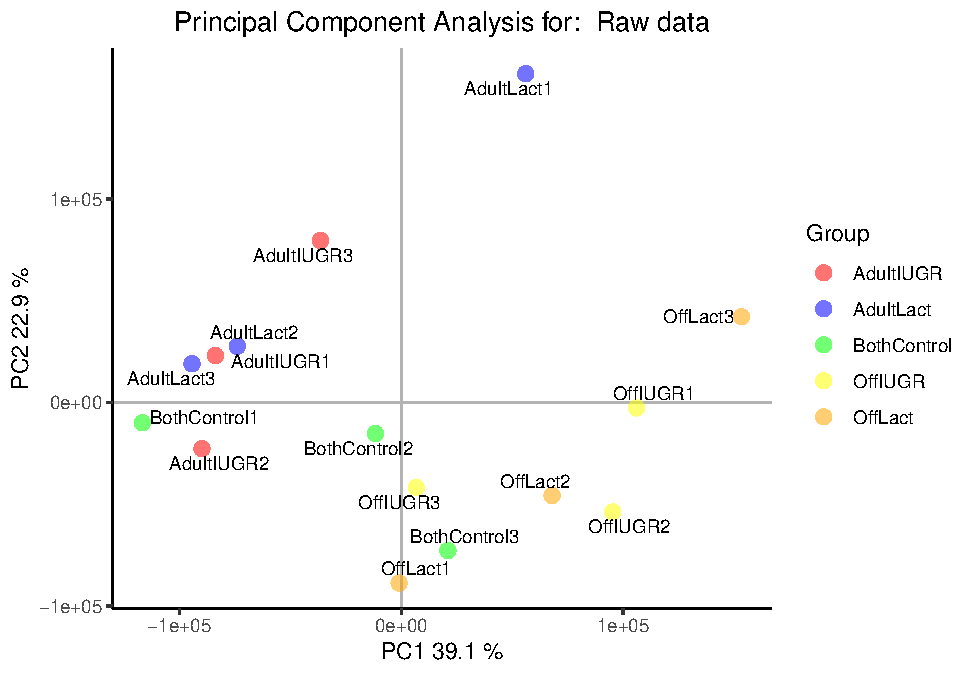
\includegraphics{delVal_AnaIsabel_ADO_PEC1_files/figure-latex/unnamed-chunk-11-1.pdf}

We save image to tiff file in figures folder.

With a boxplot we visualize the intensity distribution of the arrays.
The group legend colors are different in boxplot and PCA, so let's have
a deep look before interpretation.

\begin{Shaded}
\begin{Highlighting}[]
\KeywordTok{boxplot}\NormalTok{(rawData, }\DataTypeTok{cex.axis=}\FloatTok{0.5}\NormalTok{, }\DataTypeTok{las=}\DecValTok{2}\NormalTok{,  }\DataTypeTok{which=}\StringTok{"all"}\NormalTok{, }
\DataTypeTok{col =} \KeywordTok{c}\NormalTok{(}\KeywordTok{rep}\NormalTok{(}\StringTok{"red"}\NormalTok{, }\DecValTok{3}\NormalTok{), }\KeywordTok{rep}\NormalTok{(}\StringTok{"blue"}\NormalTok{, }\DecValTok{3}\NormalTok{), }
        \KeywordTok{rep}\NormalTok{(}\StringTok{"green"}\NormalTok{, }\DecValTok{3}\NormalTok{), }\KeywordTok{rep}\NormalTok{(}\StringTok{"yellow"}\NormalTok{, }\DecValTok{3}\NormalTok{), }\KeywordTok{rep}\NormalTok{(}\StringTok{"orange"}\NormalTok{, }\DecValTok{3}\NormalTok{))}
\NormalTok{,}\DataTypeTok{main=}\StringTok{"Distribution of raw intensity values"}\NormalTok{)}
\end{Highlighting}
\end{Shaded}

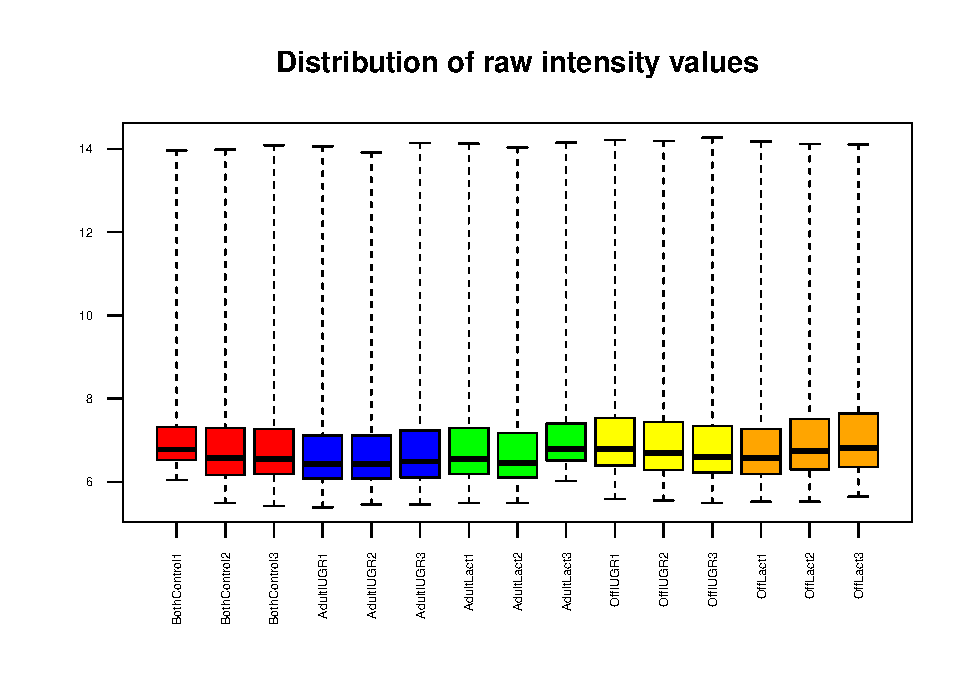
\includegraphics{delVal_AnaIsabel_ADO_PEC1_files/figure-latex/unnamed-chunk-13-1.pdf}

A light variation of intensity among arrays is observed, but this is the
expected for raw data.

\subparagraph{Data normalization}\label{data-normalization}

\begin{Shaded}
\begin{Highlighting}[]
\NormalTok{eset_rma <-}\StringTok{ }\KeywordTok{rma}\NormalTok{(rawData)}
\end{Highlighting}
\end{Shaded}

\begin{verbatim}
## Background correcting
## Normalizing
## Calculating Expression
\end{verbatim}

\subparagraph{Quality control of normalized
data}\label{quality-control-of-normalized-data}

After normalization, the array AdultLact1 has been moved to the left
part of the scatterplot.

First component of the PCA accounts for 19.3\% of the total variability.
It separates samples by the generation, as offsprings are on the right
and adults are on the left. After normalization, without exception.

\begin{Shaded}
\begin{Highlighting}[]
\KeywordTok{plotPCA3}\NormalTok{(}\KeywordTok{exprs}\NormalTok{(eset_rma), }\DataTypeTok{labels =}\NormalTok{ targets}\OperatorTok{$}\NormalTok{ShortName, }\DataTypeTok{factor =}\NormalTok{ targets}\OperatorTok{$}\NormalTok{Group, }
\DataTypeTok{title=}\StringTok{"Normalized data"}\NormalTok{, }\DataTypeTok{scale =} \OtherTok{FALSE}\NormalTok{, }\DataTypeTok{size =} \DecValTok{3}\NormalTok{, }
\DataTypeTok{colores =} \KeywordTok{c}\NormalTok{(}\StringTok{"red"}\NormalTok{, }\StringTok{"blue"}\NormalTok{, }\StringTok{"green"}\NormalTok{, }\StringTok{"yellow"}\NormalTok{,}\StringTok{"orange"}\NormalTok{))}
\end{Highlighting}
\end{Shaded}

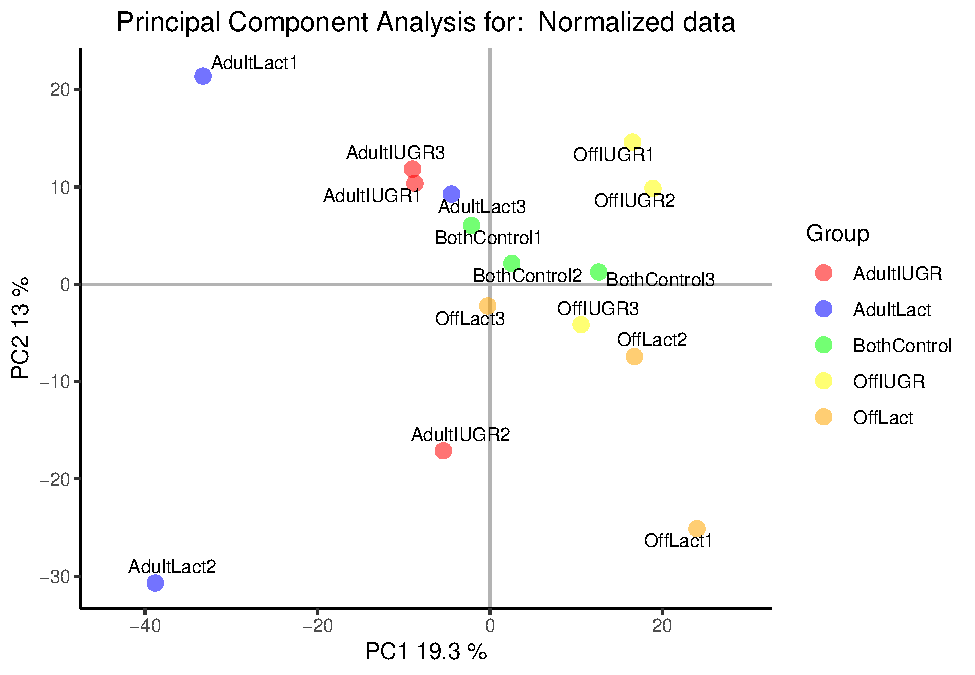
\includegraphics{delVal_AnaIsabel_ADO_PEC1_files/figure-latex/unnamed-chunk-17-1.pdf}

\begin{Shaded}
\begin{Highlighting}[]
\KeywordTok{boxplot}\NormalTok{(eset_rma, }\DataTypeTok{cex.axis=}\FloatTok{0.5}\NormalTok{, }\DataTypeTok{las=}\DecValTok{2}\NormalTok{,  }\DataTypeTok{which=}\StringTok{"all"}\NormalTok{, }
\DataTypeTok{col =} \KeywordTok{c}\NormalTok{(}\KeywordTok{rep}\NormalTok{(}\StringTok{"red"}\NormalTok{, }\DecValTok{3}\NormalTok{), }\KeywordTok{rep}\NormalTok{(}\StringTok{"blue"}\NormalTok{, }\DecValTok{3}\NormalTok{), }\KeywordTok{rep}\NormalTok{(}\StringTok{"green"}\NormalTok{, }\DecValTok{3}\NormalTok{), }\KeywordTok{rep}\NormalTok{(}\StringTok{"yellow"}\NormalTok{, }\DecValTok{3}\NormalTok{),}\KeywordTok{rep}\NormalTok{(}\StringTok{"orange"}\NormalTok{, }\DecValTok{3}\NormalTok{)),}
\DataTypeTok{main=}\StringTok{"Boxplot for arrays intensity: Normalized Data"}\NormalTok{)}
\end{Highlighting}
\end{Shaded}

\begin{verbatim}
## Warning in .local(x, ...): Argument 'which' ignored (not meaningful for ExpressionSet)
\end{verbatim}

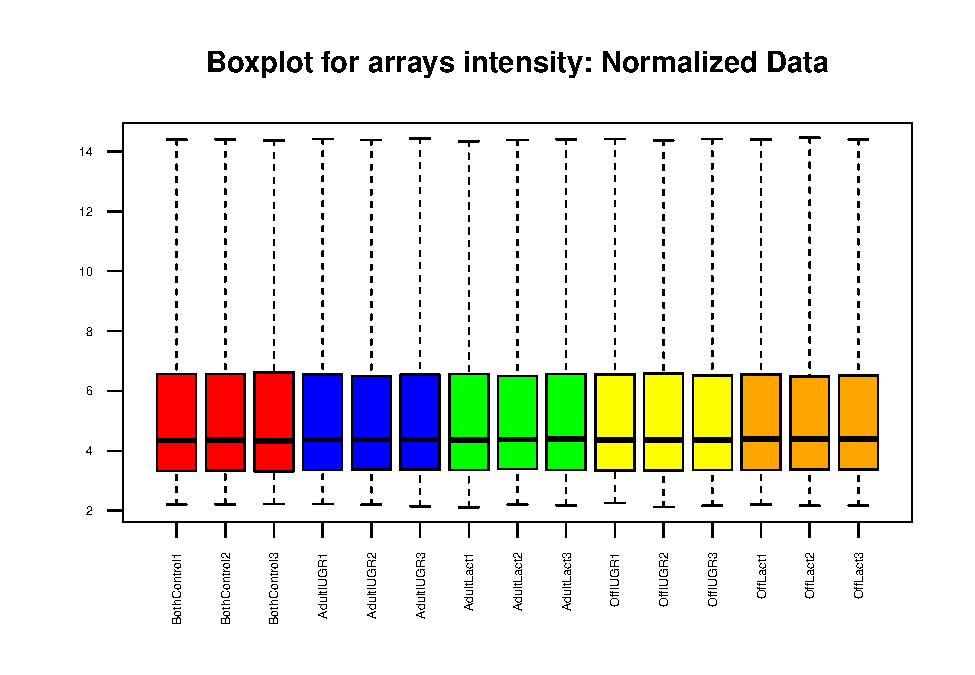
\includegraphics{delVal_AnaIsabel_ADO_PEC1_files/figure-latex/unnamed-chunk-19-1.pdf}

\subparagraph{Batch detection}\label{batch-detection}

\begin{Shaded}
\begin{Highlighting}[]
\NormalTok{bp <-}\StringTok{ }\KeywordTok{barplot}\NormalTok{(pvcaObj}\OperatorTok{$}\NormalTok{dat, }\DataTypeTok{xlab =} \StringTok{"Effects"}\NormalTok{,}
\DataTypeTok{ylab =} \StringTok{"Weighted average proportion variance"}\NormalTok{,}
\DataTypeTok{ylim=} \KeywordTok{c}\NormalTok{(}\DecValTok{0}\NormalTok{,}\FloatTok{1.1}\NormalTok{),}\DataTypeTok{col =} \KeywordTok{c}\NormalTok{(}\StringTok{"mediumorchid"}\NormalTok{), }\DataTypeTok{las=}\DecValTok{2}\NormalTok{,}
\DataTypeTok{main=}\StringTok{"PVCA estimation"}\NormalTok{)}

\KeywordTok{axis}\NormalTok{(}\DecValTok{1}\NormalTok{, }\DataTypeTok{at =}\NormalTok{ bp, }\DataTypeTok{labels =}\NormalTok{ pvcaObj}\OperatorTok{$}\NormalTok{label, }\DataTypeTok{cex.axis =} \FloatTok{0.55}\NormalTok{, }\DataTypeTok{las=}\DecValTok{2}\NormalTok{)}

\NormalTok{values =}\StringTok{ }\NormalTok{pvcaObj}\OperatorTok{$}\NormalTok{dat}

\NormalTok{new_values =}\StringTok{ }\KeywordTok{round}\NormalTok{(values , }\DecValTok{3}\NormalTok{)}

\KeywordTok{text}\NormalTok{(bp,pvcaObj}\OperatorTok{$}\NormalTok{dat,}\DataTypeTok{labels =}\NormalTok{ new_values, }\DataTypeTok{pos=}\DecValTok{3}\NormalTok{, }\DataTypeTok{cex =} \FloatTok{0.5}\NormalTok{)}
\end{Highlighting}
\end{Shaded}

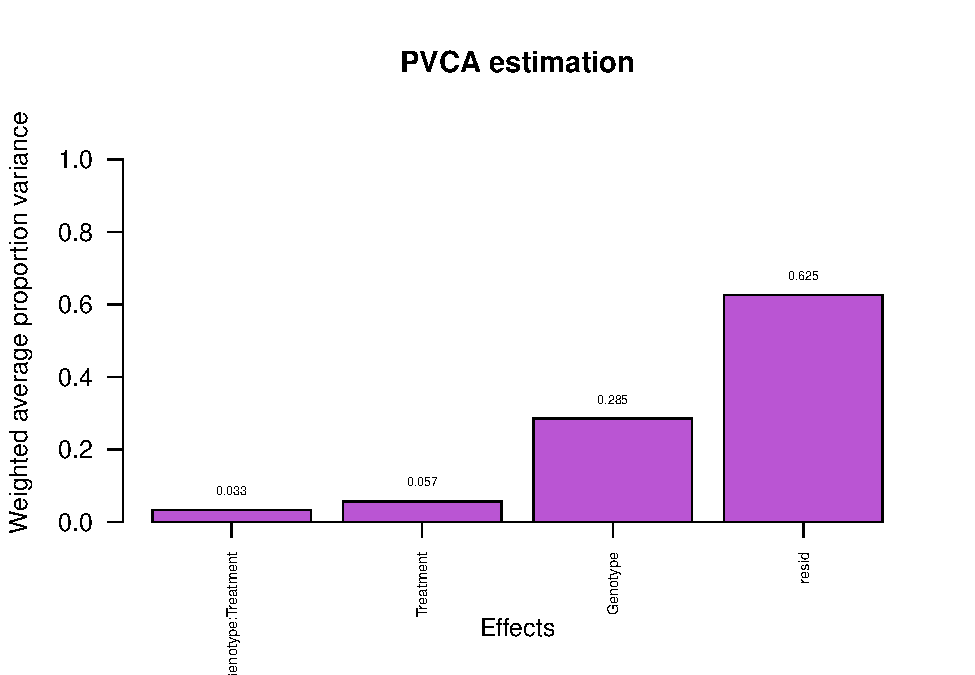
\includegraphics{delVal_AnaIsabel_ADO_PEC1_files/figure-latex/unnamed-chunk-22-1.pdf}

\subparagraph{Detecting most variable
genes}\label{detecting-most-variable-genes}

\begin{Shaded}
\begin{Highlighting}[]
\NormalTok{sds <-}\StringTok{ }\KeywordTok{apply}\NormalTok{ (}\KeywordTok{exprs}\NormalTok{(eset_rma), }\DecValTok{1}\NormalTok{, sd)}
\NormalTok{sdsO<-}\StringTok{ }\KeywordTok{sort}\NormalTok{(sds)}
\KeywordTok{plot}\NormalTok{(}\DecValTok{1}\OperatorTok{:}\KeywordTok{length}\NormalTok{(sdsO), sdsO, }\DataTypeTok{main=}\StringTok{"Distribution of variability for all genes"}\NormalTok{,}
\DataTypeTok{sub=}\StringTok{"Vertical lines represent 90% and 95% percentiles"}\NormalTok{,}
\DataTypeTok{xlab=}\StringTok{"Gene index (from least to most variable)"}\NormalTok{, }\DataTypeTok{ylab=}\StringTok{"Standard deviation"}\NormalTok{)}
\KeywordTok{abline}\NormalTok{(}\DataTypeTok{v=}\KeywordTok{length}\NormalTok{(sds)}\OperatorTok{*}\KeywordTok{c}\NormalTok{(}\FloatTok{0.9}\NormalTok{,}\FloatTok{0.95}\NormalTok{))}
\end{Highlighting}
\end{Shaded}

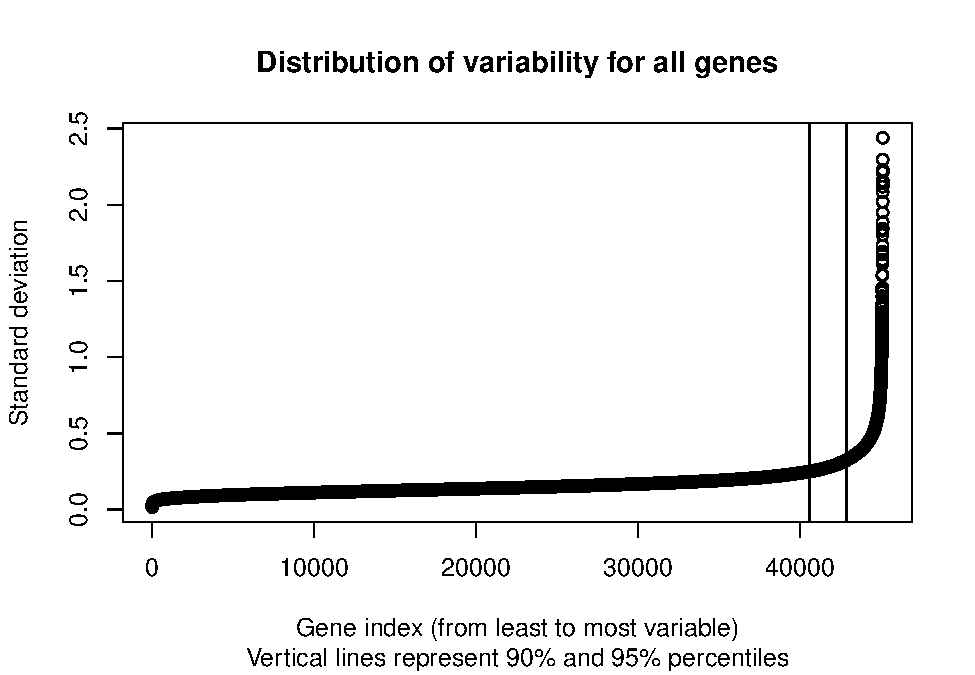
\includegraphics{delVal_AnaIsabel_ADO_PEC1_files/figure-latex/unnamed-chunk-24-1.pdf}

Values of standard deviations allong all samples for all genes ordered
from smallest to biggest

\subparagraph{Filter least variable
genes}\label{filter-least-variable-genes}

\begin{Shaded}
\begin{Highlighting}[]
\KeywordTok{print}\NormalTok{(filtered}\OperatorTok{$}\NormalTok{filter.log)}
\end{Highlighting}
\end{Shaded}

\begin{verbatim}
## $numDupsRemoved
## [1] 17422
## 
## $numLowVar
## [1] 15416
## 
## $numRemoved.ENTREZID
## [1] 7111
## 
## $feature.exclude
## [1] 13
\end{verbatim}

Before filtering, there were 45101 genes.

After filtering, there are 5139 genes left.

\subparagraph{Save normalized data}\label{save-normalized-data}

We save data in results folder.

\paragraph{3. Define the experimental
setup}\label{define-the-experimental-setup}

Compare gene expression between groups.

The Linear Models for Microarrays method, implemented in the limma
package Smyth (2005) is used to select differential expressed genes.

\subparagraph{Create the design matrix}\label{create-the-design-matrix}

The first step for the analysis based on linear models is to create the
design matrix. Basically it is a table that describes the allocation of
each sample to a group or experimental condition. It has as many rows as
samples and as many columns as groups (if only one factor is
considered). Each row contains a one in the column of the group to which
the sample belongs and a zero in the others.

1 model of 1 factor with 5 levels defined in Targets\textgreater{}Groups
\textgreater{} 5 columns.

\begin{Shaded}
\begin{Highlighting}[]
\NormalTok{designMat<-}\StringTok{ }\KeywordTok{model.matrix}\NormalTok{(}\OperatorTok{~}\DecValTok{0}\OperatorTok{+}\NormalTok{Group, }\KeywordTok{pData}\NormalTok{(eset_filtered))}
\KeywordTok{colnames}\NormalTok{(designMat) <-}\StringTok{ }\KeywordTok{c}\NormalTok{(}\StringTok{"BothControl"}\NormalTok{, }\StringTok{"AdultIUGR"}\NormalTok{, }\StringTok{"AdultLact"}\NormalTok{, }\StringTok{"OffIUGR"}\NormalTok{,}\StringTok{"OffLact"}\NormalTok{)}
\end{Highlighting}
\end{Shaded}

\subparagraph{Defining comparisons with the Contrasts
Matrix}\label{defining-comparisons-with-the-contrasts-matrix}

It consists of as many columns as comparisons and as many rows as groups
(that is, as columns of the design matrix) -\textgreater{} (5rows by 3
columns).

A comparison between groups - called ``contrast'' - is represented by a
``1'' and a ``-1'' in the rows of groups to compare and zeros in the
rest.

3 comparisons \textgreater{} 3 columns in the contrast matrix.

Build the contrast matrix that can be used to answer the following
questions:

\begin{itemize}
\item
  Compare the effect of IntraUterine Growth Restriction in offsprings.
\item
  Compare the effect of overfed during lactation in offsprings.
\item
  The interaction: the differences between the two previous effects in
  offsprings.
\end{itemize}

There could be more comparisons to be made, but I have highlighted here
which I consider the most interesting ones.

\begin{Shaded}
\begin{Highlighting}[]
\NormalTok{cont.matrix <-}\StringTok{ }\KeywordTok{makeContrasts}\NormalTok{ (}\DataTypeTok{BothControlvsOffIUGR =}\NormalTok{ BothControl}\OperatorTok{-}\NormalTok{OffIUGR,}
                              \DataTypeTok{BothControlvsOffLact =}\NormalTok{ BothControl}\OperatorTok{-}\NormalTok{OffLact,}
                              \DataTypeTok{INT =}\NormalTok{ OffIUGR }\OperatorTok{-}\StringTok{ }\NormalTok{OffLact,}\DataTypeTok{levels=}\NormalTok{designMat)}
\KeywordTok{print}\NormalTok{(cont.matrix)}
\end{Highlighting}
\end{Shaded}

\begin{verbatim}
##              Contrasts
## Levels        BothControlvsOffIUGR BothControlvsOffLact INT
##   BothControl                    1                    1   0
##   AdultIUGR                      0                    0   0
##   AdultLact                      0                    0   0
##   OffIUGR                       -1                    0   1
##   OffLact                        0                   -1  -1
\end{verbatim}

\subparagraph{Model estimation and gene
selection}\label{model-estimation-and-gene-selection}

With LIMMA, once the design matrix and the contrasts have been defined,
we can proceed to estimate the model, estimate the contrasts and perform
the significance tests that will lead to the decision, for each gene and
each comparison, if they can be considered differential expressed.

The analysis provides the usual test statistics such as Fold-change
t-moderated or adjusted p-values that are used to order the genes from
more unless differential expressed.

In order to control the percentage of false positives that may result
from high number of contrasts made simultaneously the p-values are
adjusted so that we have control over the false positive rate using the
Benjamini and Hochberg method Benjamini and Hochberg (1995).

topTable: for a given contrast a list of genes ordered from smallest to
biggest p--value which can be considered to be most to least
differential expressed.

For Comparison 1:

\begin{Shaded}
\begin{Highlighting}[]
\NormalTok{topTab_BothControlvsOffIUGR <-}\StringTok{ }
\StringTok{  }\KeywordTok{topTable}\NormalTok{(fit.main, }
           \DataTypeTok{number=}\KeywordTok{nrow}\NormalTok{(fit.main),}
           \DataTypeTok{coef=}\StringTok{"BothControlvsOffIUGR"}\NormalTok{,}
           \DataTypeTok{adjust=}\StringTok{"fdr"}\NormalTok{) }
\KeywordTok{head}\NormalTok{(topTab_BothControlvsOffIUGR)}
\end{Highlighting}
\end{Shaded}

\begin{verbatim}
##                 logFC  AveExpr         t      P.Value   adj.P.Val         B
## 1438758_at -2.3282725 7.522021 -7.667917 1.420024e-06 0.007297503 4.6330862
## 1450064_at -0.9691825 5.919838 -5.544024 5.565138e-05 0.123768511 1.8148609
## 1439059_at -1.3650712 3.503159 -5.351001 8.006620e-05 0.123768511 1.5192822
## 1417600_at  0.9120025 6.368973  5.207271 1.053043e-04 0.123768511 1.2950501
## 1415685_at -0.6306643 8.318089 -5.026904 1.490648e-04 0.123768511 1.0088038
## 1440771_at -1.6306961 5.828590 -4.991487 1.596670e-04 0.123768511 0.9519765
\end{verbatim}

For Comparison 2:

\begin{Shaded}
\begin{Highlighting}[]
\NormalTok{topTab_BothControlvsOffLact <-}\StringTok{ }
\StringTok{  }\KeywordTok{topTable}\NormalTok{(fit.main, }
           \DataTypeTok{number=}\KeywordTok{nrow}\NormalTok{(fit.main), }
           \DataTypeTok{coef=}\StringTok{"BothControlvsOffLact"}\NormalTok{, }
           \DataTypeTok{adjust=}\StringTok{"fdr"}\NormalTok{) }
\KeywordTok{head}\NormalTok{(topTab_BothControlvsOffLact)}
\end{Highlighting}
\end{Shaded}

\begin{verbatim}
##                   logFC  AveExpr         t      P.Value  adj.P.Val        B
## 1431182_at   -2.1237194 6.235149 -6.270831 1.479835e-05 0.03736404 3.074858
## 1421061_at    0.7838334 4.975084  6.084998 2.062107e-05 0.03736404 2.797971
## 1418243_at   -1.0436027 7.227763 -5.890252 2.934492e-05 0.03736404 2.501370
## 1420634_a_at  1.3477017 6.054184  5.888456 2.944129e-05 0.03736404 2.498604
## 1427357_at    1.2081038 7.753155  5.773408 3.635341e-05 0.03736404 2.320273
## 1433966_x_at -2.4863124 4.070717 -5.651317 4.556100e-05 0.03902299 2.128548
\end{verbatim}

For Comparison 3:

\begin{Shaded}
\begin{Highlighting}[]
\NormalTok{topTab_INT <-}\StringTok{ }
\StringTok{  }\KeywordTok{topTable}\NormalTok{(fit.main, }
  \DataTypeTok{number=}\KeywordTok{nrow}\NormalTok{(fit.main), }
  \DataTypeTok{coef=}\StringTok{"INT"}\NormalTok{, }
  \DataTypeTok{adjust=}\StringTok{"fdr"}\NormalTok{) }
\KeywordTok{head}\NormalTok{(topTab_INT)}
\end{Highlighting}
\end{Shaded}

\begin{verbatim}
##                  logFC   AveExpr         t      P.Value  adj.P.Val        B
## 1438758_at    2.091071  7.522021  6.886719 5.097879e-06 0.02619800 3.652820
## 1421225_a_at  1.033863  8.182224  6.153676 1.823124e-05 0.04684518 2.678164
## 1428636_at   -1.541085  5.162313 -5.658011 4.499814e-05 0.05895101 1.964637
## 1424041_s_at -1.001887 11.290039 -5.589442 5.112300e-05 0.05895101 1.862482
## 1460467_at    1.151154  5.162744  5.512947 5.898825e-05 0.05895101 1.747545
## 1424351_at   -1.497486  7.095931 -5.430945 6.882780e-05 0.05895101 1.623196
\end{verbatim}

First column of each topTable contains the manufacturer's (Affymetrix)
ID for each probeset. Next step is to guess which gene correspond to
each Affymetrix ID. This process is called annotation. Gene Symbol, the
Entrez Gene identifier or the Gene description.

Annotation tables, one per comparison.

Let's see for the first comparison:

\begin{Shaded}
\begin{Highlighting}[]
\NormalTok{short_BothControlvsOffIUGR <-}\StringTok{ }\KeywordTok{head}\NormalTok{(topAnnotated_BothControlvsOffIUGR[}\DecValTok{1}\OperatorTok{:}\DecValTok{5}\NormalTok{,}\DecValTok{1}\OperatorTok{:}\DecValTok{4}\NormalTok{]) }
\NormalTok{short_BothControlvsOffIUGR}
\end{Highlighting}
\end{Shaded}

\begin{verbatim}
##      PROBEID SYMBOL ENTREZID                                        GENENAME
## 1 1415673_at   Psph   100678                       phosphoserine phosphatase
## 2 1415685_at  Mtif2    76784 mitochondrial translational initiation factor 2
## 3 1415698_at  Golm1   105348                        golgi membrane protein 1
## 4 1415743_at  Hdac5    15184                           histone deacetylase 5
## 5 1415750_at   Tbl3   213773                        transducin (beta)-like 3
\end{verbatim}

\subparagraph{Visualizating differential
expression}\label{visualizating-differential-expression}

The names of the top 4 genes are shown in blue in the figure.

This is for BothControlvsOffIUGR comparison.

\begin{Shaded}
\begin{Highlighting}[]
\KeywordTok{volcanoplot}\NormalTok{(fit.main, }\DataTypeTok{coef=}\DecValTok{1}\NormalTok{, }\DataTypeTok{highlight=}\DecValTok{4}\NormalTok{, }\DataTypeTok{names=}\NormalTok{SYMBOLS, }
\DataTypeTok{main=}\KeywordTok{paste}\NormalTok{(}\StringTok{"Differentially expressed genes"}\NormalTok{, }\KeywordTok{colnames}\NormalTok{(cont.matrix)[}\DecValTok{1}\NormalTok{], }\DataTypeTok{sep=}\StringTok{"}\CharTok{\textbackslash{}n}\StringTok{"}\NormalTok{))}
\KeywordTok{abline}\NormalTok{(}\DataTypeTok{v=}\KeywordTok{c}\NormalTok{(}\OperatorTok{-}\DecValTok{1}\NormalTok{,}\DecValTok{1}\NormalTok{))}
\end{Highlighting}
\end{Shaded}

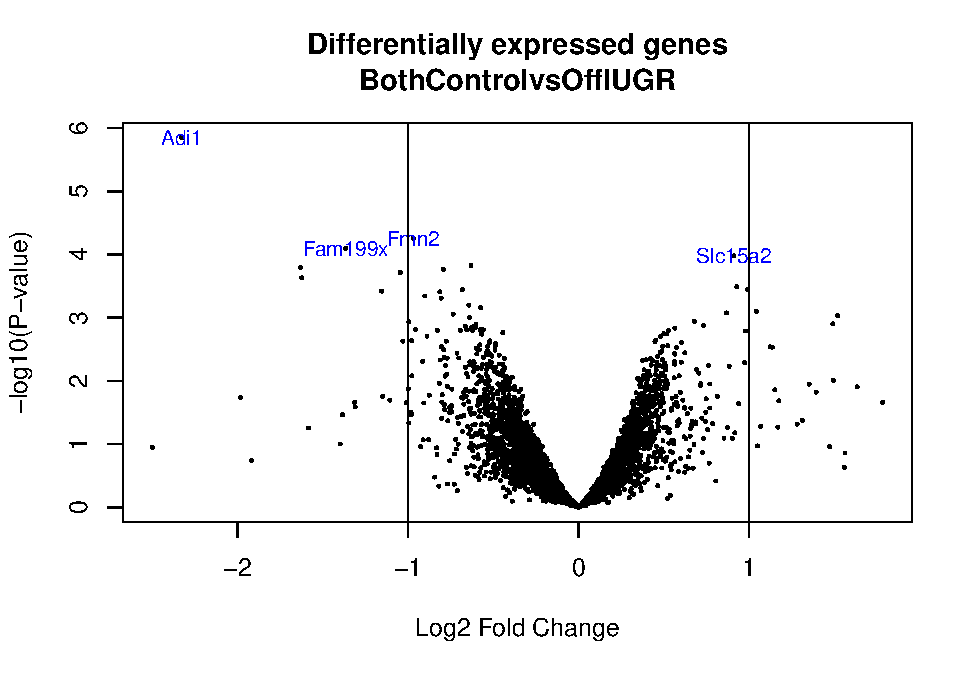
\includegraphics{delVal_AnaIsabel_ADO_PEC1_files/figure-latex/unnamed-chunk-43-1.pdf}

For second comparison BothControlvsOffLact:

\begin{Shaded}
\begin{Highlighting}[]
\KeywordTok{volcanoplot}\NormalTok{(fit.main, }\DataTypeTok{coef=}\DecValTok{2}\NormalTok{, }\DataTypeTok{highlight=}\DecValTok{4}\NormalTok{, }\DataTypeTok{names=}\NormalTok{SYMBOLS, }
\DataTypeTok{main=}\KeywordTok{paste}\NormalTok{(}\StringTok{"Differentially expressed genes"}\NormalTok{, }\KeywordTok{colnames}\NormalTok{(cont.matrix)[}\DecValTok{2}\NormalTok{], }\DataTypeTok{sep=}\StringTok{"}\CharTok{\textbackslash{}n}\StringTok{"}\NormalTok{))}
\KeywordTok{abline}\NormalTok{(}\DataTypeTok{v=}\KeywordTok{c}\NormalTok{(}\OperatorTok{-}\DecValTok{1}\NormalTok{,}\DecValTok{1}\NormalTok{))}
\end{Highlighting}
\end{Shaded}

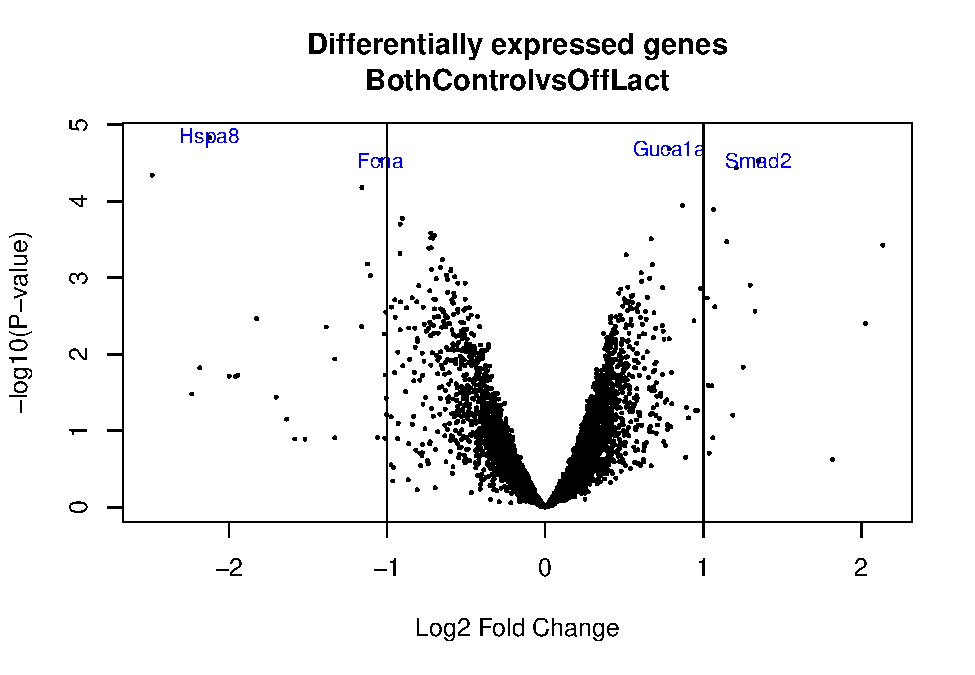
\includegraphics{delVal_AnaIsabel_ADO_PEC1_files/figure-latex/unnamed-chunk-45-1.pdf}

For third comparison INT:

\begin{Shaded}
\begin{Highlighting}[]
\KeywordTok{volcanoplot}\NormalTok{(fit.main, }\DataTypeTok{coef=}\DecValTok{3}\NormalTok{, }\DataTypeTok{highlight=}\DecValTok{4}\NormalTok{, }\DataTypeTok{names=}\NormalTok{SYMBOLS, }
\DataTypeTok{main=}\KeywordTok{paste}\NormalTok{(}\StringTok{"Differentially expressed genes"}\NormalTok{, }\KeywordTok{colnames}\NormalTok{(cont.matrix)[}\DecValTok{3}\NormalTok{], }\DataTypeTok{sep=}\StringTok{"}\CharTok{\textbackslash{}n}\StringTok{"}\NormalTok{))}
\KeywordTok{abline}\NormalTok{(}\DataTypeTok{v=}\KeywordTok{c}\NormalTok{(}\OperatorTok{-}\DecValTok{1}\NormalTok{,}\DecValTok{1}\NormalTok{))}
\end{Highlighting}
\end{Shaded}

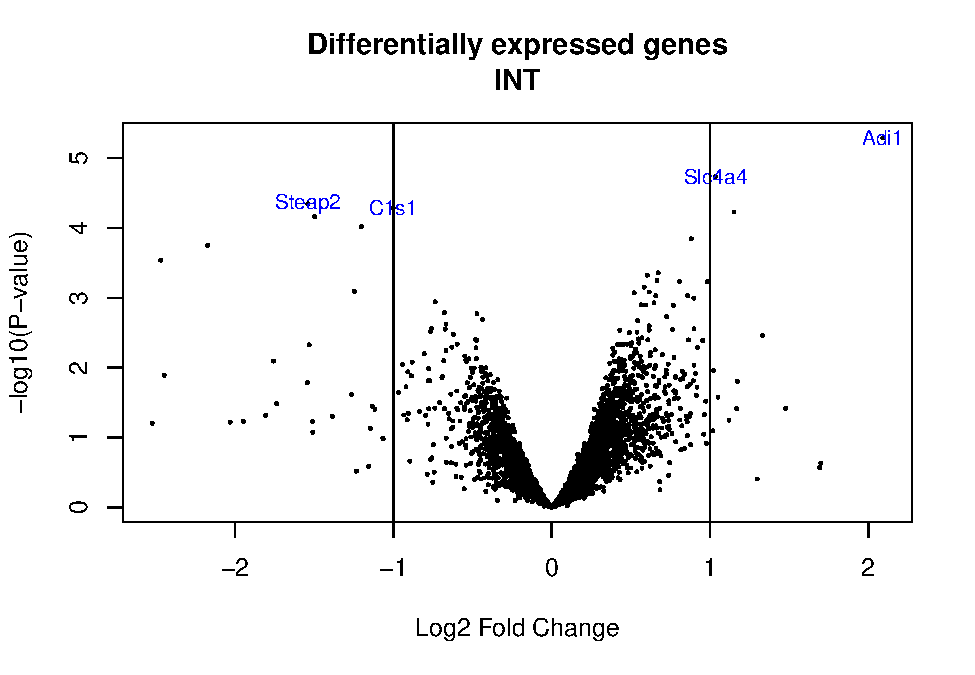
\includegraphics{delVal_AnaIsabel_ADO_PEC1_files/figure-latex/unnamed-chunk-47-1.pdf}

\subparagraph{Multiple comparisons}\label{multiple-comparisons}

When one selects genes in several comparisons it is usually interesting
to know which genes have been selected in each comparison. Sometimes
biologically relevant genes will be those that are selected in one of
them but not in others. In other occasions he interest will lie in genes
that are selected in all comparisons.

This object has as many columns as comparisons and as many rows as
genes: 5139x3.

Per each gene and comparison a ``+1'' denotes significantly up-regulated
(t-test values \textgreater{}0, FDR \textless{} selected cutoff), a
``-1'' significantly down-regulated (t-test values \textless{}0, FDR
\textless{} selected cutoff) and a ``0'' non significant difference (FDR
\textgreater{} selected cutoff).

\begin{Shaded}
\begin{Highlighting}[]
\NormalTok{sum.res.rows<-}\KeywordTok{apply}\NormalTok{(}\KeywordTok{abs}\NormalTok{(res),}\DecValTok{1}\NormalTok{,sum)}
\NormalTok{res.selected<-res[sum.res.rows}\OperatorTok{!=}\DecValTok{0}\NormalTok{,] }
\KeywordTok{print}\NormalTok{(}\KeywordTok{summary}\NormalTok{(res))}
\end{Highlighting}
\end{Shaded}

\begin{verbatim}
##        BothControlvsOffIUGR BothControlvsOffLact  INT
## Down                      1                    4    4
## NotSig                 5138                 5132 5132
## Up                        0                    3    3
\end{verbatim}

This can be visualized in a Venn Diagram.

\begin{Shaded}
\begin{Highlighting}[]
\KeywordTok{vennDiagram}\NormalTok{ (res.selected[,}\DecValTok{1}\OperatorTok{:}\DecValTok{3}\NormalTok{], }\DataTypeTok{cex=}\FloatTok{0.9}\NormalTok{)}
\KeywordTok{title}\NormalTok{(}\StringTok{"Genes in common between the three comparisons}\CharTok{\textbackslash{}n}\StringTok{ Genes selected with FDR < 0.1 and logFC > 1"}\NormalTok{)}
\end{Highlighting}
\end{Shaded}

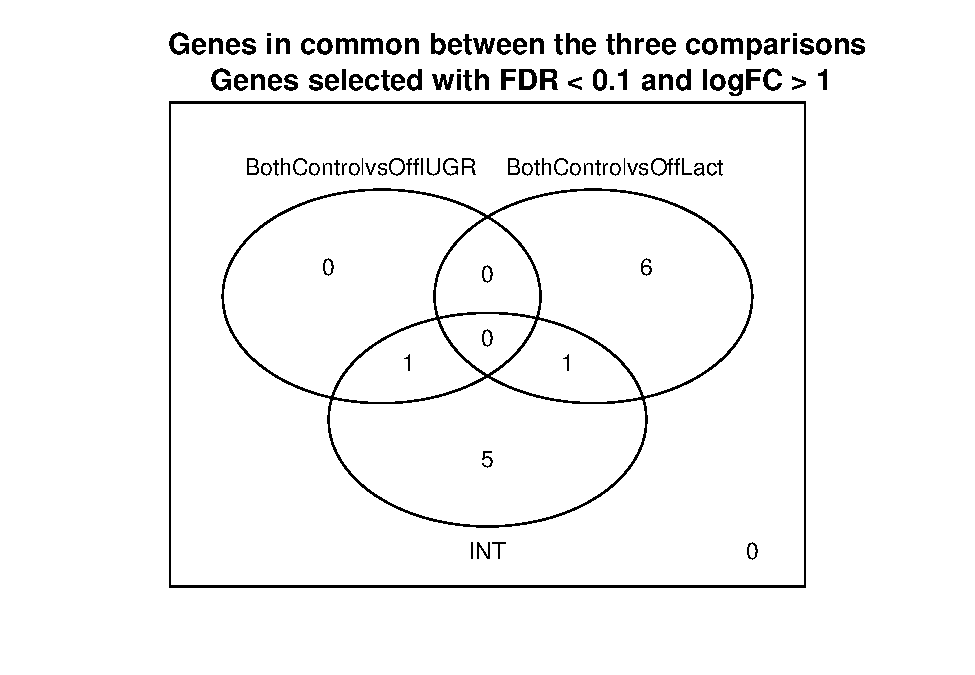
\includegraphics{delVal_AnaIsabel_ADO_PEC1_files/figure-latex/unnamed-chunk-51-1.pdf}

Venn diagram showing the genes in common between the three comparisons
performed.

\paragraph{4. Expression profiles visualization:
Heatmaps}\label{expression-profiles-visualization-heatmaps}

Genes that have been selected as differential expressed may be
visualized using a heatmap. These plots use color palettes to highlight
distinct values --here positive (up-regulation) or negative
(down-regulation) significantly differential expressions.

Heatmaps can be used to visualize the expression values of differential
expressed genes with no specific order, but it is usually preferred to
plot them doing a hierarchical clustering on genes (rows) or
columns(samples) in order to find groups of genes with common patterns
of variation which can eventually be associated to the different groups
being compared.

A common option is to select the gens that have been selected in the
previous steps, that is the genes that have been called differential
expressed in at least one comparison.

(FDR \textless{} 0.1 and logFC \textgreater{} 1)

\begin{Shaded}
\begin{Highlighting}[]
\NormalTok{my_palette <-}\StringTok{ }\KeywordTok{colorRampPalette}\NormalTok{(}\KeywordTok{c}\NormalTok{(}\StringTok{"blue"}\NormalTok{, }\StringTok{"red"}\NormalTok{))(}\DataTypeTok{n =} \DecValTok{299}\NormalTok{)}
 
\KeywordTok{heatmap.2}\NormalTok{(HMdata,}
\DataTypeTok{Rowv =} \OtherTok{FALSE}\NormalTok{,}
\DataTypeTok{Colv =} \OtherTok{FALSE}\NormalTok{,}
\DataTypeTok{main =} \StringTok{"Differentially expressed genes }\CharTok{\textbackslash{}n}\StringTok{ FDR < 0,1, logFC >=1"}\NormalTok{,}
\DataTypeTok{scale =} \StringTok{"row"}\NormalTok{,}
\DataTypeTok{col =}\NormalTok{ my_palette,}
\DataTypeTok{sepcolor =} \StringTok{"white"}\NormalTok{,}
\DataTypeTok{sepwidth =} \KeywordTok{c}\NormalTok{(}\FloatTok{0.05}\NormalTok{,}\FloatTok{0.05}\NormalTok{),}
\DataTypeTok{cexRow =} \FloatTok{0.5}\NormalTok{,}
\DataTypeTok{cexCol =} \FloatTok{0.9}\NormalTok{,}
\DataTypeTok{key =} \OtherTok{TRUE}\NormalTok{,}
\DataTypeTok{keysize =} \FloatTok{1.5}\NormalTok{,}
\DataTypeTok{density.info =} \StringTok{"histogram"}\NormalTok{,}
\DataTypeTok{ColSideColors =} \KeywordTok{c}\NormalTok{(}\KeywordTok{rep}\NormalTok{(}\StringTok{"red"}\NormalTok{,}\DecValTok{3}\NormalTok{),}\KeywordTok{rep}\NormalTok{(}\StringTok{"blue"}\NormalTok{,}\DecValTok{3}\NormalTok{), }\KeywordTok{rep}\NormalTok{(}\StringTok{"green"}\NormalTok{,}\DecValTok{3}\NormalTok{), }\KeywordTok{rep}\NormalTok{(}\StringTok{"yellow"}\NormalTok{,}\DecValTok{3}\NormalTok{),}\KeywordTok{rep}\NormalTok{(}\StringTok{"orange"}\NormalTok{,}\DecValTok{3}\NormalTok{)),}
\DataTypeTok{tracecol =} \OtherTok{NULL}\NormalTok{,}
\DataTypeTok{dendrogram =} \StringTok{"none"}\NormalTok{,}
\DataTypeTok{srtCol =} \DecValTok{30}\NormalTok{)}
\end{Highlighting}
\end{Shaded}

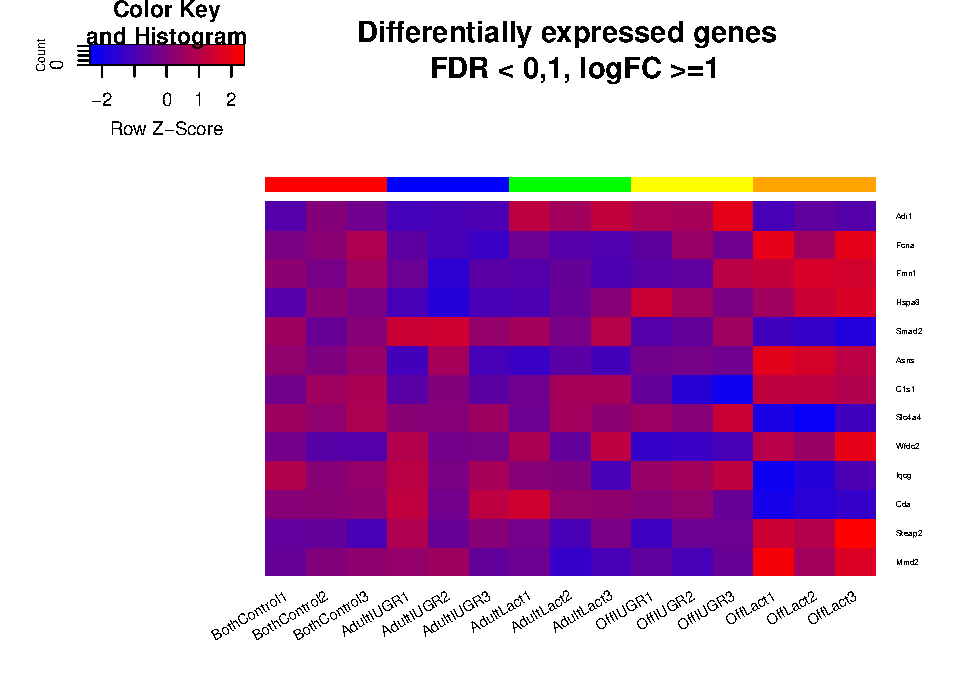
\includegraphics{delVal_AnaIsabel_ADO_PEC1_files/figure-latex/unnamed-chunk-54-1.pdf}

Genes and samples are forced to group by row and column similarity
respectively.

\begin{Shaded}
\begin{Highlighting}[]
\KeywordTok{heatmap.2}\NormalTok{(HMdata,}
\DataTypeTok{Rowv =} \OtherTok{TRUE}\NormalTok{,}
\DataTypeTok{Colv =} \OtherTok{TRUE}\NormalTok{,}
\DataTypeTok{dendrogram=}\StringTok{"both"}\NormalTok{,}
\DataTypeTok{main =} \StringTok{"Differentially expressed genes }\CharTok{\textbackslash{}n}\StringTok{ FDR < 0,1, logFC >=1"}\NormalTok{,}
\DataTypeTok{scale =} \StringTok{"row"}\NormalTok{,}
\DataTypeTok{col =}\NormalTok{ my_palette,}
\DataTypeTok{sepcolor =} \StringTok{"white"}\NormalTok{,}
\DataTypeTok{sepwidth =} \KeywordTok{c}\NormalTok{(}\FloatTok{0.05}\NormalTok{,}\FloatTok{0.05}\NormalTok{),}
\DataTypeTok{cexRow =} \FloatTok{0.5}\NormalTok{,}
\DataTypeTok{cexCol =} \FloatTok{0.9}\NormalTok{,}
\DataTypeTok{key =} \OtherTok{TRUE}\NormalTok{,}
\DataTypeTok{keysize =} \FloatTok{1.5}\NormalTok{,}
\DataTypeTok{density.info =} \StringTok{"histogram"}\NormalTok{,}
\DataTypeTok{ColSideColors =} \KeywordTok{c}\NormalTok{(}\KeywordTok{rep}\NormalTok{(}\StringTok{"red"}\NormalTok{,}\DecValTok{3}\NormalTok{),}\KeywordTok{rep}\NormalTok{(}\StringTok{"blue"}\NormalTok{,}\DecValTok{3}\NormalTok{), }\KeywordTok{rep}\NormalTok{(}\StringTok{"green"}\NormalTok{,}\DecValTok{3}\NormalTok{), }\KeywordTok{rep}\NormalTok{(}\StringTok{"yellow"}\NormalTok{,}\DecValTok{3}\NormalTok{),}\KeywordTok{rep}\NormalTok{(}\StringTok{"orange"}\NormalTok{,}\DecValTok{3}\NormalTok{)),}
\DataTypeTok{tracecol =} \OtherTok{NULL}\NormalTok{,}
\DataTypeTok{srtCol =} \DecValTok{30}\NormalTok{)}
\end{Highlighting}
\end{Shaded}

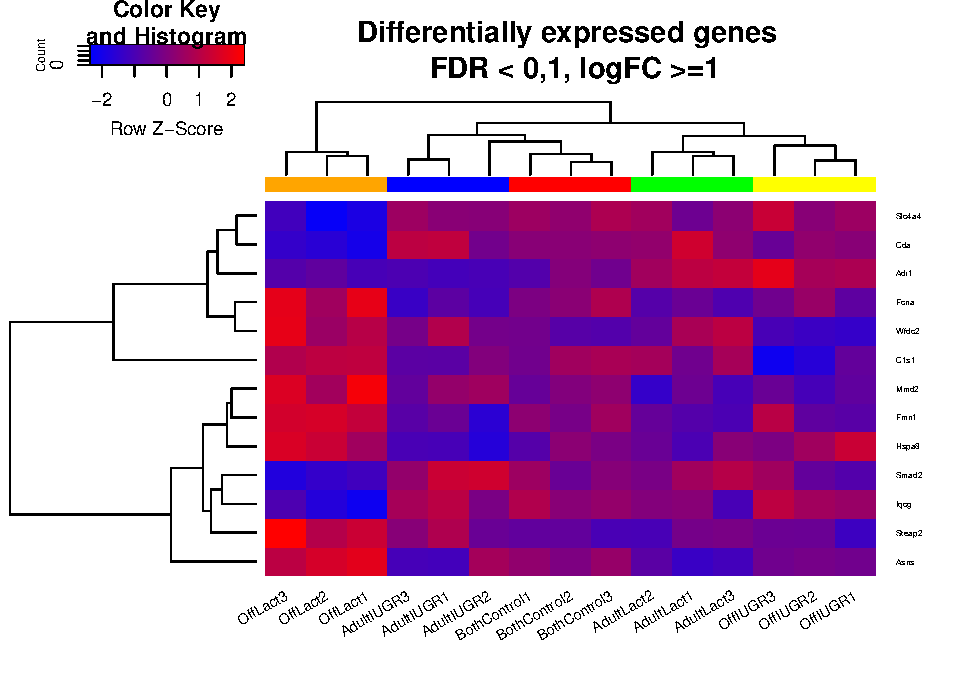
\includegraphics{delVal_AnaIsabel_ADO_PEC1_files/figure-latex/unnamed-chunk-56-1.pdf}

\subsection{Biological Significance of
results}\label{biological-significance-of-results}

Given a list of genes selected for being differential expressed between
two conditions, the functions, biological processes or molecular
pathways that characterize them appear on this list more frequently than
among the rest of the genes analyzed.

ReactomePA Bioconductor package. The analysis is done on the ReactomePA
annotation database \url{https://reactome.org/}.

Analyses of this type need a minimum number of genes to be reliable,
preferably a few hundreds than a few dozens, so it is common to perform
a selection less restrictive than with the previous steps. For instance
an option is to include all genes with a non-stringent FDR cutoff, such
as FDR \textless{} 0.15 without filtering by minimum ``fold-change'').

The analysis also requires to have the Entrez Identifiers for all genes
analyzed. It is an open discussion if what one should use is ``all genes
analyzed'' -that is genes that have been retained in the analysis and
are part of the ``topTable''- or all genes available. In this case we
use the second option and define our universe to be all genes that have
at least one annotation in the Gene Ontology.

The Biological significance analysis will be applied to these lists:
``BothControlvsOffLact'' ``INT''.

First rows and columns for Reactome results on INT.csv comparison:

\begin{Shaded}
\begin{Highlighting}[]
\NormalTok{Tab.react <-}\StringTok{ }\KeywordTok{read.csv2}\NormalTok{(}\KeywordTok{file.path}\NormalTok{(}\StringTok{"./results/ReactomePA.Results.INT.csv"}\NormalTok{), }\DataTypeTok{sep =} \StringTok{","}\NormalTok{, }\DataTypeTok{header =} \OtherTok{TRUE}\NormalTok{, }\DataTypeTok{row.names =} \DecValTok{1}\NormalTok{)}

\NormalTok{Tab.react <-}\StringTok{ }\NormalTok{Tab.react[}\DecValTok{1}\OperatorTok{:}\DecValTok{4}\NormalTok{, }\DecValTok{1}\OperatorTok{:}\DecValTok{4}\NormalTok{]}
\NormalTok{knitr}\OperatorTok{::}\KeywordTok{kable}\NormalTok{(Tab.react, }\DataTypeTok{booktabs =} \OtherTok{TRUE}\NormalTok{, }\DataTypeTok{caption =} \StringTok{"First rows and columns for Reactome results on INT.csv comparison"}\NormalTok{)}
\end{Highlighting}
\end{Shaded}

\begin{table}

\caption{\label{tab:unnamed-chunk-61}First rows and columns for Reactome results on INT.csv comparison}
\centering
\begin{tabular}[t]{lllll}
\toprule
  & Description & GeneRatio & BgRatio & pvalue\\
\midrule
R-MMU-71291 & Metabolism of amino acids and derivatives & 2/5 & 200/8698 & 0.0050257698525165\\
R-MMU-2162123 & Synthesis of Prostaglandins (PG) and Thromboxanes (TX) & 1/5 & 12/8698 & 0.00688070797551199\\
R-MMU-1614635 & Sulfur amino acid metabolism & 1/5 & 20/8698 & 0.0114467660674098\\
R-MMU-917977 & Transferrin endocytosis and recycling & 1/5 & 31/8698 & 0.0176976576334369\\
\bottomrule
\end{tabular}
\end{table}

This netwowrk figure shows the network produced from the genes selected
in the comparison

\begin{Shaded}
\begin{Highlighting}[]
\KeywordTok{cnetplot}\NormalTok{(enrich.result, }\DataTypeTok{categorySize =} \StringTok{"geneNum"}\NormalTok{, }\DataTypeTok{schowCategory =} \DecValTok{15}\NormalTok{, }
\DataTypeTok{vertex.label.cex =} \FloatTok{0.75}\NormalTok{)}
\end{Highlighting}
\end{Shaded}

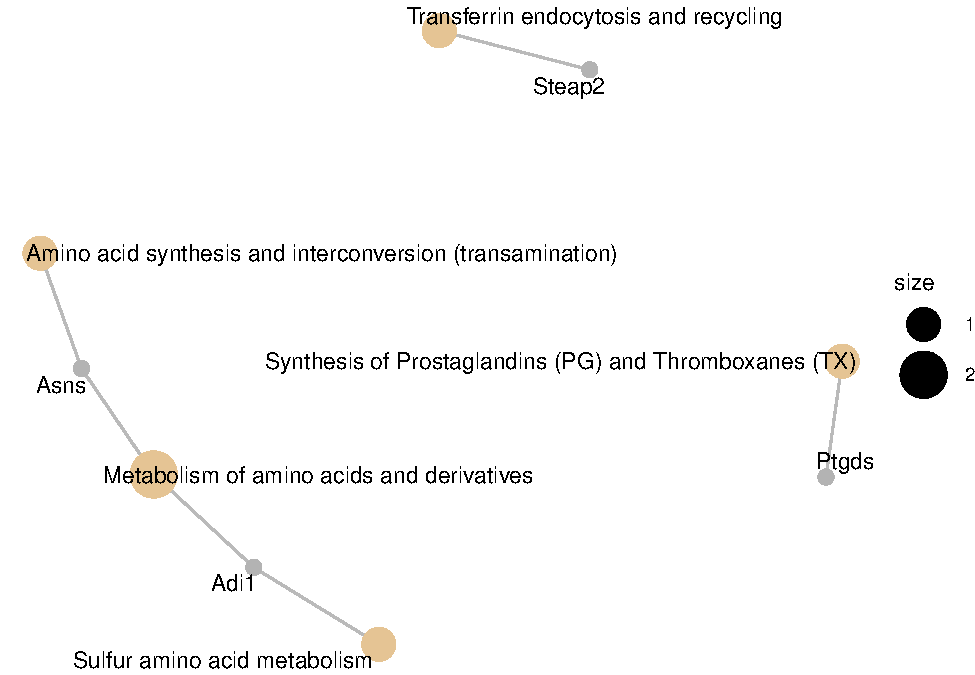
\includegraphics{delVal_AnaIsabel_ADO_PEC1_files/figure-latex/unnamed-chunk-62-1.pdf}

In comparison INT, 8 enriched pathways have been found, for example:
Sulfur amino acid metabolism.

The results obtained in the analysis of biological significance are:

\begin{itemize}
\item
  a .csv file with a summary of all the enriched pathways and the
  associated statistics.
\item
  a bar plot with the best enriched pathways. Height of the bar plot is
  the number of genes of our analysis related with that pathway.
  Moreover, pathways are ordered by statistical significance.
\item
  a plot with a network of the enriched pathways and the relation among
  the genes included.
\end{itemize}

\subsection{Discussion}\label{discussion}

I have found a limitation in comparison BothControlvsOffIUGR. There was
not enriched pathway found so Reactome results on this comparison was
NULL.

For future iterations of this study, we could think of other comparisons
such as:

\begin{itemize}
\item
  Compare the effect of IntraUterine Growth Restriction in adults.
\item
  Compare the interaction of IntraUterine Growth Restriction in adults
  and offsprings.
\item
  Compare the effect of overfed during lactation in adults.
\item
  Compare the interaction of overfed during lactation in adults and
  offsprings.
\end{itemize}

\subsection{Apendix}\label{apendix}

The code can be found in the Github repository, in .RMd file, where the
reproducibility of the study is guaranteed.

\end{document}
